\chapter{Algoritmers Udførelsestid}
\label{ch:Algoritmers Udførelsestid}

\section{Tid som Funktion af \red{Argumentets } Kardinalitet}
\label{sec:Tid som Funktion af Argumentets Kardinalitet}

Dette afsnit bygger primært på side $24$ og $25$ i bogen \emph{"Algoritmer og Datastrukturer"} \cite{aogd}.\\

Når vi analyserer algoritmer, er det primære formål at skabe udsagn, der kort og præcist beskriver algoritmers opførsel. I vores tilfælde er vi interesserede i algoritmens udførselsestid. Vi lader $\I _n$ være mængden af mulige argumenter til algoritmen, $n$ være kardinaliteten (størrelsen) af $\I _n$ og $I$ være en instans af $\I$ (altså $I \in \I _n$). Algoritmens udførselsestid $T$ når kan nu beskrives som funktion af instansen $T(I)$. Vi kan bruge dette til at beskrive tre egenskaber af algoritmens udførselsestid: algoritmens maksimale udførselsestid, algoritmens minimale udførselsestid og algoritmens gennemsnitlige køretid. Den maksimale udførselsestid er udførselsestid ved det værste tilfælde ($T(I_{værst})$), den minimale udførselsestid kan modsat beskrives som køretiden på det bedste tilfælde ($T(I_{bedst})$), og den gennemsnitlige udførselsestid kan findes ved at tage gennemsnittet af alle udførselsestiderne ($\frac{1}{|\I |} \sum_{I \in \I _n}T(I)$). Med disse udtryk kan vi nu opskrive algoritmens mulige udførselsestider som funktion af kardinaliteten $n$ af $\I _n$ således:

\[ T(n) = \left\{ \begin{array}{l}
	T(I_{værst}): I_{værst} \in \I _n  \\
	T(I_{bedst}): I_{bedst} \in \I _n  \\
	\frac{1}{|\I _n|} \sum_{I \in \I _n}T(I)
\end{array} \right.\s\s\begin{array}{l}
	\text{værste tilfælde}\\
	\text{bedste tilfælde}\\
	\text{i gennemsnit}
\end{array}\]

Alle disse størrelser beskriver et aspekt af algoritmens udførselsestid, dog er den mest interessante udførselsestiden i værste tilfælde. Det er samme koncept som når postvæsnet siger at det vil tage tre bankdage for din pakke at nå frem, selvom det godt kan ske hurtigere. Det værste tilfælde \emph{garanterer} at hvornår algoritmen er færdig. Dette værste tilfælde kan sammen med det bedste tilfælde bestemme variansen på udførselsestiden. Hvis en algoritme viser stor varians i dens udførselsestid kan gennemsnitsudførselsestiden sige noget om hvordan man kan forvente at algoritmen opfører sig.\\

Denne form for algoritmeanalyse er dog ikke helt problemfri: for det første kan vi aldrig definere nogen fast forskrift for $T(n)$, der ville gøre det muligt at beregne den præcise udførselsestid. Dette kan tildels forklares af Allan Turings "halt problem" [\red{kilde}] hvor han viste at man aldrig kan vide om en algoritme stopper eller ender i en uendelig lykke. Problemet med at kunne bestemme en køretid for algoritmen er at man så ville vide at algoritmen stoppede før den havde kørt. En anden forflaring er at alle computere vil køre den samme algoritme i forskellig hastighed pga. varians i computerens komponenter. Derudover vil selv den samme computer aldrig udføre en handling i præcis samme tidsinterval, da andre processer på computeren kan bruge dele af computerens ydeevne, eller fordi at cpu'ens temperatur ændre sig. Der er mange faktorer der bestemme hvor lang tid det tager en algoritme at fuldføre, hvilket gør det meget svært at denne form for analyse praktisk.\\

Uanset hvilken forklaring man bruger, er det svært at sige meget om den faktiske køretid for en algoritme før man har kørt algoritmen. Derfor er det nemmere, og mere brugbart at forfolde sig til udførselsestidens vækstrate og algoritmens opførsel når $n$ bliver meget stort. Denne form for analyse hedder store-O-analyse.

\section{\red{Store-O-Analyse}}
\label{sec:Store-O-Analyse}

I store-O-analyse forholder vi os til hvordan udførselsestidens stiger, når $n$ bliver meget stort. I denne form for analyse indeler vi grupper efter deres vækstrate. En funktions vækstrate beskriver hvor hurtigt en funktion stiger i forhold til andre funktioner ved meget høje $n$-værdier. Hvis en funktion $f(n)$ har en højere vækstrate end funktionen $g(x)$, betyder det at funktionen $f(x)$ altid vil være større end $g(x)$ ved store nok $n$. Det har ingenbetydning om $f(n)$ er mindre end $g(n)$ ved små $n$, da $f(n)$ altid vil overstige $g(n)$ pga. dens højere vækstrate. Matematisk kan man sige at an funktion $f(n))$ har en højere vækstrate end $g(n)$, hvis n $f(n) \geq c \cdot g(n)$  (hvor $c$ er en konstant, og $n$ er tilstrækkeligt stort). Hvis funktionerne har \emph{samme} vækstrate gælder det at $c \leq \frac{f(n)}{g(n)} \leq d$ \red{[skal jeg have den med?] }(hvor $d$ er en konstant, og det samme gælder for $n$ og $c$ som før). I praksis betyder dette at funktioner som $n^2$ og $n^2+3n-10$ har den samme vækstrate og, at den er højere end en funktion som $n \cdot log(n)$. Vi kan nu bruge disse regler til at definere store-O-notattion (se figur \ref{fig:Store-O definition}). Lad os begynde med $O(f(n))$. En funktion er del af mængden $O(f(n))$, hvis den kan sættes ind som $g(n)$. Med den matematiske definition menes der: $g(n)$ skal være sådan at (:) der findes en værdi $c$, som er større end $0$, sådan at (:) der findes et positivt helt tal $n_0$, sådan at der for alle $n$ større end $n_0$, gælder at $g(n)$ er mindre eller lig $c \cdot f(n)$, dvs. $g(n)$ har mindre eller samme vækstrate som $f(n))$. I praksis betyder dette, at der altid vil være en positiv $n_0$, hvorefter $f(n)$ altid vil være højere end eller lig $g(n)$ (se figur \ref{fig:Store-o og n2}). Man kan også tænke mængden $O(f(n))$ som mængden af funktioner der \emph{ikke vokser hurtigere end} $f(n)$.\\

Når man siger at en algoritme er $O(n^2)$, menes der altså at vækstraten for $T(n)$ er en del af mængden $O(n^2)$, og at $T(n)$ i værste tilfælde har samme vækstrate som $n^2$.\\

$\Omega (f(n))$ indeholder modsat $O(f(n))$ alle funktioner der vokser mindst lige så hurtigt som $f(n)$.\\

Der er dog en vækstrate som både $O(f(n))$ og $\Omega (f(n))$ indeholder: nemlig vækstraten af $f(n)$.For at beskrive \emph{præcis} denne mængde funktioner bruger vi $\Theta (n)$. Hvis en algoritme er $\Theta (n^3)$ betyder det altså at $T(n)$ \emph{altid} vil have samme vækstrate som $n^3$. Det ville også betyde at alle input af samme kardinalitet vil resultere lige lang udførselsestid.

\section{Kompleksetetsklasser}
\label{sec:Kompleksetetsklasser}


%Grunden til dette, er at algoritmeoptimering (hvor man bruger meget algoritmeanalyse) netop har størst effekt hvis algoritmens input har en høj kardinalitet.

\begin{figure}
	\begin{center}
		\padtable
		\begin{tabular}{l}
			\hline
			$O(f(n)) = {g(n): \exists c > 0: \exists n_0 \in \N_+: \forall n \geq n_0: g(n) \leq c \cdot f(n)}$\\
			$\Omega (f(n)) = {g(n): \exists c > 0: \exists n_0 \in \N_+: \forall n \geq n_0: g(n) \geq c \cdot f(n)}$\\
			$\Theta (f(n)) = O(f(n)) \cup \Omega (f(n))$\\
			\hline
		\end{tabular}
	\end{center}
	%\vspace{-3mm}
	\caption{Definition af $O(f(n))$, $\Omega (f(n))$ og $\Theta (f(n))$ \cite[s. 26]{aogd}.}
	\label{fig:Store-O definition}
\end{figure}

\begin{figure}
	\begin{center}
		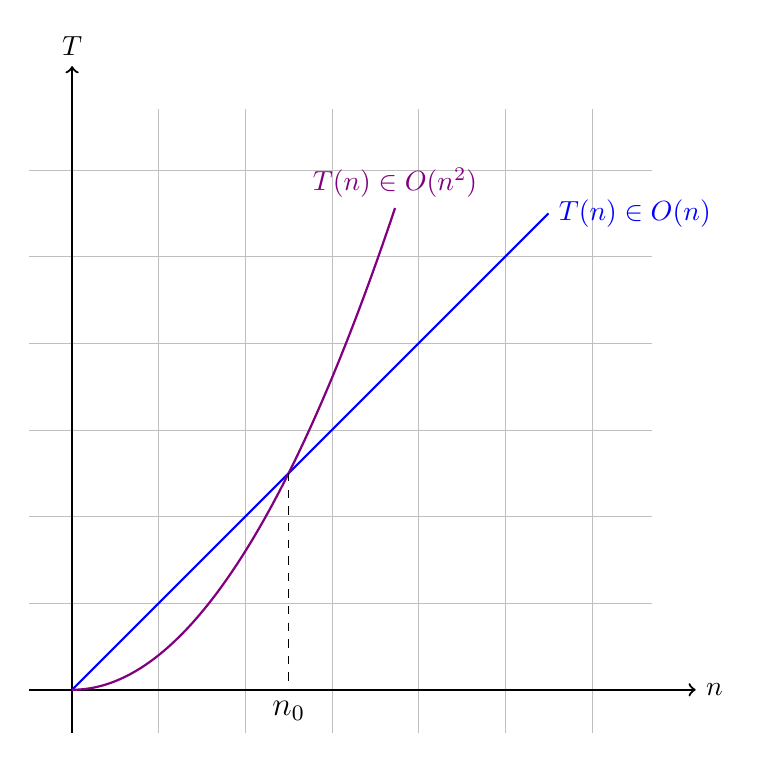
\begin{tikzpicture}[domain=0:7,range=0:3,scale=1.1] 
			\normalsize
			\coordinate (I) at (2.5,2.5);
			\coordinate (I0) at (2.5,0);
			\draw[very thin,color=lightgray] (-0.5,-0.5) grid (6.7,6.7);
			\draw[thick,->] (-0.5,0) -- (7.2,0) node[right] {$n$}; \draw[thick,->] (0,-0.5) -- (0,7.2) node[above] {$T$};
			\draw[thick,color=blue, samples=150,domain=0:5.5]	plot (\x,{\x})	node[right] {$T(n) \in O(n)$}; 
			\draw[thick,color=violet, samples=150,domain=0:3.73]	plot (\x,{0.4*\x^2})	node[above] {$T(n) \in O(n^2)$}; 
			\large
			\draw[dashed] (I) -- (I0) node[below] {$n_0$};
		\end{tikzpicture}
		%\includegraphics[scale=0.5]{../img/Store-o og n0.png}
	\end{center}
	\caption{Her ses skæringspunktet $n_0$, hvorefter $g(n)$ altid er højere end $f(n)$. Altså vækstraten af $g(n)$ højere end vækstraten af $f(n)$.}
	%  \cite{n0}
	\label{fig:Store-o og n2}
\end{figure}



